\documentclass[12pt]{article}
\usepackage[T1]{fontenc}
%\usepackage[latin9]{inputenc}
\usepackage[utf8]{inputenc}
\usepackage[english]{babel}
\usepackage{amsmath}
%\usepackage{halloweenmath}
\usepackage{amsfonts}
\usepackage{amssymb}
%\usepackage{setspace}
\usepackage{rotating}
\usepackage{graphics}
\usepackage{eurosym}
\usepackage[round]{natbib}
%\usepackage{graphicx}
%\usepackage{float} 				%allows you to float images
\usepackage{latexsym}
%\usepackage{bbding}
%\usepackage {moresize}
\usepackage{listings}
\usepackage{bbding}
\usepackage{blindtext}
\usepackage{hhline}
\usepackage{tikz}
\usetikzlibrary{trees}
%\usetikzlibrary{shapes,backgrounds}
%\usepackage{pgfplots}
%\usetikzlibrary{arrows}
\usepackage{enumitem}
%\doublespacing
%\usepackage{geometry}
\usepackage{amsthm}
\usepackage{color}
%\usepackage{array,multirow}
\usepackage{subcaption}
%\usepackage{pst-plot}
%	\psset{xunit=15mm}
%\geometry{verbose,tmargin=1in,bmargin=1in,lmargin=.5in,rmargin=.5in}
\setlength{\parskip}{\bigskipamount}
\setlength{\parindent}{0pt}
\usepackage{multicol}


\newenvironment{problem}[3][Problem]{\begin{trivlist}
\item[\hskip \labelsep {\bfseries #1}\hskip \labelsep {\bfseries #2.}]}{\end{trivlist}}

\newcommand{\barr}{\bar{r}}
\newcommand{\ddx}{\frac{d}{dx}}
\newcommand{\infsum}{\sum_{n=1}^{\infty }}

\title{Problem Set 13 \thanks{Problems:19.2, 19,10, 19.11, 19.24}}
\author{Ian McGroarty \\
	Course Number: 555.444 \\
}
\date{November 25, 2019}

\begin{document}

\maketitle
%%%%%%%%%%%%%%%%%%%%%%%%%%%%%%%%%%%%%%%%%%%%%%%%%%%%%%%%
%%%%%%%%%%%%%%%%%%%%%%%%%%%%%%%%%%%%%%%%%%%%%%%%%%%%%%%%
%%%%%%%%%%%%%%%%%%%%%%%%%%%%%%%%%%%%%%%%%%%%%%%%%%%%%%%%

\newpage
\begin{problem}{19.2}. What does it mean to assert that the delta of a call option is 0.7? How can a short position in 1,000 options be made delta neutral when the delta of each option in 0.7.

The delta of an option is defined as the rate of change of th option price with respect to the asset price. When the delta of a call option is 0.7. It means that a dollar increase in the asset price is associated with a change of around \$0.70 in the option price. Hedgers can use this information to protect against changes in the asset price. An investor who sold 1000 options can hedge their position bu purchasing $0.7 \cdot 1000 = 700$ shares of the asset. 
\end{problem}

\begin{problem}{19.10}. Find the delta of a short position on 1000 European Call options on silver futures. The options mature in 8 months, and the futures contract underlying he option matures in nine months. $F_0 =\$ 8.00 , K = \$ 8.00 ,  r = 0.12, \sigma = 0.18$. 

First we calculate $d_1$ using the BSM for futures products (pg. 388). Then using table 19.6 (pg. 419) we can calculate the delta of the futures option with q equal to the risk free rate, r. We find $\Delta = 0.4886$ so the delta of the short position is $(0.4886 * 1000 = -488.6$. Note to self that it is negative because it is a short position!
\begin{align*}
d_1 &= \frac{ln(F_0/K) + (\sigma^2/2)(T)}{\sigma \sqrt{T}}  && \text{(pg 388)} \\
d_1 &= 0.07348 \\
N(d_1) &= 0.5293 \\
delta &= e^{-qT}N(d_1) && \text{Table 19.6 pg 419} \\
&= 0.4886
\end{align*}
\end{problem}

\begin{problem}{19.11}. What initial position in nine month silver futures is necessary for delta hedging? If silver itself is used what is the initial position? If one-year silver futures are used what is the initial position? 

A delta of -488.6 means that the investor will need to purchase 489 shares in order to hedge initially. But that is based only on the nine month silver futures contract. If the investor wanted to buy silver, then we essentially need to do the forward price looking forward nine months assuming no storage costs and interest at the risk free rate. So $489\cdot e^{0.12 \cdot 0.75} = 535.0512$ Therefore, the investor could hedge using 535 (ounces?) of silver. Finally, the one year futures value can be calculated by discounting the silver position one year; $535\cdot e^{-0.12} = 474.5$. Thus, the investor could hedge using 475 one year silver futures options. 
\end{problem}

\begin{problem}{19.24}. First lets calculate the delta of the portfolio: 
$$ (-1000 \cdot 0.5) + (-500 \cdot 0.8) + (-2000 \cdot -0.4) + (-500 \cdot 0.70) = -450 $$
This means that the portfolio can be made delta neutral by buying 450 shares of sterling. Now to calculate the gamma of the portfolio:
$$ (-1000 \cdot 2.2) + (-500 \cdot 0.6) + (-2000 \cdot 1.3) + (-500 \cdot 1.8) = -6000 $$
The portfolio can be made gamma neutral by taking a long position of $\frac{6000}{1.5} = 4000$ in the traded option. This action will change the delta of the portfolio from 0 to $4000\cdot 0.7 = 2800$. There fore 2800 units of the sterling will make it delta neutral again. Thus, to make a delta and gamma neutral portfolio, the investor will want to take a long position in 4000 units of the traded option and take a short position in 2350 shares of sterling.

Now lets calculate the vega of the portfolio:
$$ (-1000 \cdot 1.8) + (-500 \cdot 0.2) + (-2000 \cdot 0.7) + (-500 \cdot 1.4) = -4000 $$
The portfolio can thus be made Vega neutral by taking a long position in $\frac{4000}{0.8} = 5000$ units of the traded option. This adds $5000 \cdot 0.7 = 3500$ to the delta, which can be offset by selling 3500 units of sterling. In sum, to make a delta and vega neutral portfolio the investor will want to buy 5000 units of the traded option and take a short position in 3050 units of sterling! 
\end{problem}
\end{document}
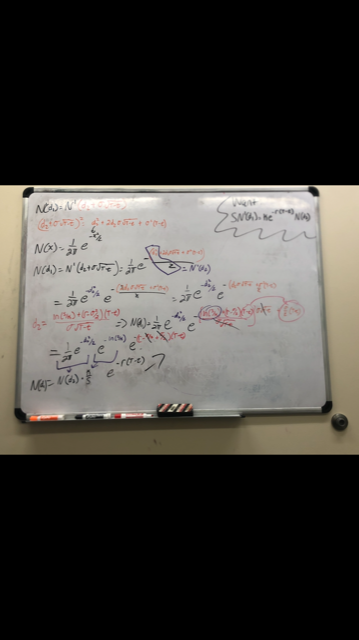
\includegraphics[width=\linewidth]{mod11_p1517b.png}

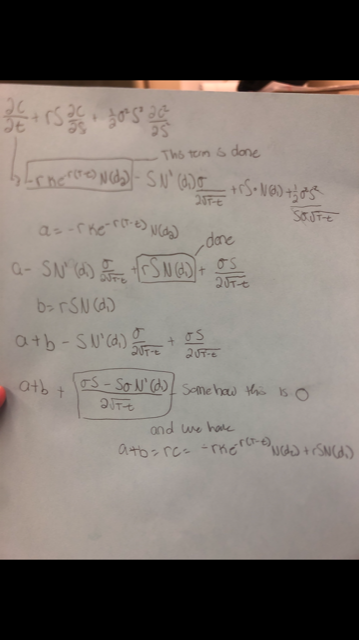
\includegraphics[width=\linewidth]{mod11_p1517f.png}
